\documentclass[a4,french,12pt]{article}
\usepackage[utf8]{inputenc}
\usepackage[T1]{fontenc}
\usepackage[french]{babel}
\usepackage[colorlinks=true,linkcolor=blue,urlcolor=blue,unicode=true]{hyperref}
\usepackage[pdftex]{graphicx}
\usepackage{amsmath}
\usepackage{amssymb}

\newcommand{\HRule}{\rule{\linewidth}{0.5mm}}

\hypersetup{
  pdftitle={Rapport TX52}
}

\begin{document}


\begin{titlepage}
\begin{center}
% Upper part of the page

% Title
\HRule \\[0.4cm]
{ \huge \bfseries Déploiement des agents composant une Smart Grid dans des micro-contrôleurs}\\[0.4cm]
 
\HRule \\[1.5cm]
%\includegraphics[width=0.60\textwidth]{images/real6410.jpg}\\[1.5cm]
% Author and supervisor
\begin{minipage}{0.4\textwidth}
\begin{flushleft} \large

%autheurs
Nicolas \textsc{Ennaji} \\
Sylvain \textsc{Marchand} 

\end{flushleft}
\end{minipage}

\vfill 
% Bottom of the page
{\large TX52 - UTBM - A11}

\end{center}
\end{titlepage}

%Sommaire
\tableofcontents

\newpage

\section{Installation et prise en main de la carte Real6410}
\subsection{Installation du kernel linux et de l'interface graphique}
Une première installation de la carte a été faite en suivant les indications de la documentation. Avec cette configuration 
l'écran n'était pas reconnu. \\
Nous avons alors recompilé le bootloader, et le kernel, afin que le driver soit intégré dans le kernel. Nous avons alors 
réussit à faire fonctionner l'écran en mode pas tactile. \\
Finalement, nous avons réinstallé le bootloader, le kernel, et qtopia en mode par défaut, mais en remplaçant le fichier 
\texttt{bootloader\_mmc} indiqué dans la documentation, par le fichier \texttt{bootloader}. Le fichier mmc permet en fait de booter depuis la 
carte SD, tandis que l'autre est fait pour booter depuis la flash de la carte. %Nous avons fait une version modifiée de la 
%documentation, simplifiée et corrigée pour installer la carte sans problème (pour une configuration de base) avec l'écran :
%Howto\_install\_linuxReal6410.pdf .\\
\subsection{Prise en main de la carte}
Nous avons commencé par créer et tester un programme de base, utilisant des sockets tcp, afin de tester la communication entre 
la carte et un ordinateur ``classique''. Grâce au système linux de la carte, ceci c'est fait sans problème. \\
Les programmes pour la cartes sont cross-comilé, donc compilé depuis un ordinateur x86, avec \texttt{arm-linux-gcc}. Cette 
variante de ggc pour processeurs ARM s'utilise exactement de la même façon qu'un gcc classique. Nous avons alors fait un 
\texttt{Makefile} pour le projet de la manière qu'on l'aurait fait pour compiler pour une machine x86. \\
Nous avons aussi pu avoir accèss à la carte par telnet. Au départ cette connection était possible sans aucune authentification 
en root. Nous avons donc ajouté un mot de passe (peu sécurisé) : root.

\newpage
\section{La communication}
\subsection{IA - Real6410}

\subsection{Real6410 - matériel}
\subsubsection{Le bus CAN}
Afin de communiquer entre la carte Real6410 et le matériel, la solution choisi est le bus CAN (Control Area Network). Cette 
solution a été choisie en raison de sa tolérence aux interférences, et de la possibilité de pouvoir relié des noeuds même 
éloignés. \\
Le bus CAN est implémenté sur la carte Real6410, il y a même un driver dans le noyau linux. De l'autre côté, une carte 
basée sur un dsPIC33F permet de piloter les batteries, et supercapacités. Le module eCAN du pic est utilisé pour 
communiquer avec la carte ARM. Nous avons donc implémenté la communication par bus CAN sur la carte PIC, et la carte ARM, 
le pilotage en des batteries quant à lui est fait par un technicien de GESC. \\
Le bus CAN est basé sur un système de messages avec un identifiant (standard ou étendu), chaque message envoyé est transmit 
à tous les noeuds du réseau, et chaque noeud récupère seulement les messages avec les identifiants qu'ils souhaites. Cette 
particularité permettra par la suite de différencier les différents types de matériels présent sur la smart grid 
(producteur, consommateurs, stockage).

\subsubsection{Côté Real6410}

\subsubsection{Côté Matériel}
Du côté matériel, on utilise le module eCAN du dsPIC33F, pour communiquer avec la carte qui supportera l'IA. Pour ce faire, 
on utilise un composant (le mcp2551) qui permet de transformer du spi en CAN. Grâce au module eCAN, nous pouvons 
``facilement'' utiliser le bus CAN. \\
La spécificité du bus CAN avec ce PIC est qu'il utilise de la DMA afin de lire et écrire les buffers d'entrée/sortie. Cela 
demande un peu de configuration, mais permet d'économiser des ressources pour le processeur. \\
Les fonction suivante ont été implémentées, afin d'être utiliser pour la communication.
\begin{itemize}
\item \texttt{void initOSC()} : Initilise l'horloge du PIC pour pouvoir maitriser la vitesse du bus CAN.
\item \texttt{void initECAN(int mode, unsigned long id)} : Initialise le bus CAN en mode mode (normal, loopback...) avec un buffer 
  en envoi et un en réception. Le buffer de réception reçoit les messages avec l'identifiant id.
\item \texttt{void initDMA()} : Initialise le buffer DMA, pour l'envoi et la réception de paquets.
\item \texttt{void sendMsg(unsigned long id, char buf[8], unsigned char canFrameType)} : envoie le message contenu dans 
  buf avec l'identifiant id, du type (standard ou étendu).
\item \texttt{void recvMsg(unsigned char bufNbr, unsigned long* id, char rcv[8])} : Réception d'un message. L'identifiant 
  est retourné dans id, et le message est copié dans rcv.
\end{itemize}
Pour le moment les identifiants ne peuvent être que standards. Il y a possibilité d'utiliser de interruptions, mais cela 
n'a pas été testé. Pour ce faire il faut appeler \texttt{void initInterrupt()}, et compléter la fonction d'interruption : 
\texttt{void \_\_attribute\_\_((interrupt, no\_auto\_psv))\_C1Interrupt(void)}.

\newpage
\section{Résultats}
\subsection{Bus CAN sur le dsPIC33F}
Les captures d'écran qui suivent, montrent dans le debbuger les resultats obtenu pour la communication par le bus CAN en mode 
loopback. \\
\\
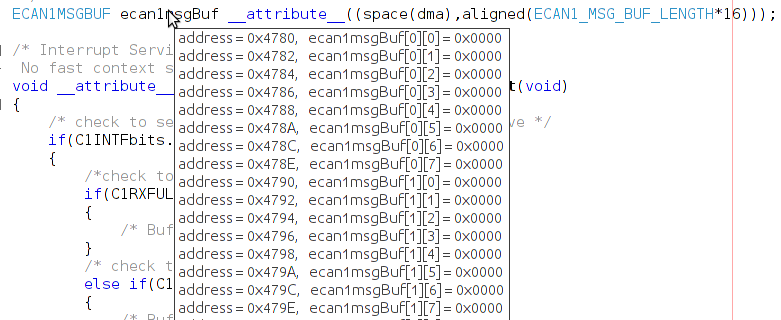
\includegraphics[width=0.8\textwidth]{images/CAN_avant_envoi.png}\\
\\
%\caption{Etat des buffers d'envoi et de réception avant l'envoi des données}
\\
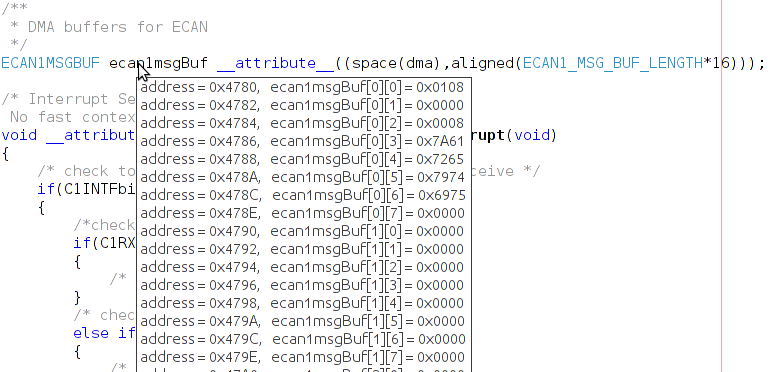
\includegraphics[width=0.8\textwidth]{images/CAN_avant_reception.png}\\
%\caption{Etat des buffers d'envoi et de réception avant réception des données}
\\
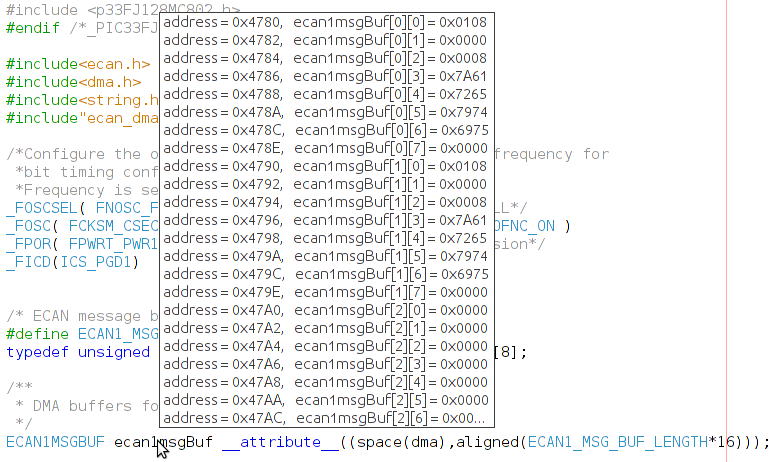
\includegraphics[width=0.8\textwidth]{images/CAN_apres_reception.png}\\
%\caption{Etat des buffers d'envoi et de réception après réception des données}
\\
On peut voir par ces captures, que dans un premier temps le buffer d'envoi (le 0) est vide. Ensuite celui ci est rempli par 
la fonction \texttt{sendMsg}. Avant que le bit de requète de l'envoi ne soit mis à 1 (à la fin de la fonction \texttt{sendMsg}), 
le buffer de réception reste vide. Les données sont ensuite reçues dans ce buffer, comme le montre la dernière capture.

\newpage
%sources si il en faut
\section{Bibliographie}

\end{document}
